\section{Feynman Diagramm}

Having introduced Gell-Mann and Low theorem, the only left is how to calculate the expectation values of time-ordered operators in Eq \ref{greenexp}.
In this section, we will show how to use a diagrammatic approach to calculate them with the help of Wicki's theorem.

However, since we have mentioned that all perturbation theory gives the same result, one way wonder why do we need such a strange approach?
Then answer is the algebraic way to calculate perturbation terms is so complicated that it is difficult to understand what does it represent for.
In contrast, Feynman diagrams give a simple visualization of what would otherwise be an arcane and abstract formula.
As David Kaiser writes, "since the middle of the 20th century, theoretical physicists have increasingly turned to this tool to help them undertake critical calculations", and so "Feynman diagrams have revolutionized nearly every aspect of theoretical physics". \cite{kaiser}

Before introducing Wick's theorem, let's first have an observation of the expression we want to calculate:
\begin{equation}
	\langle\Phi_{0}|
	\hat{\mathcal{T}} \left[ c_u^{\dagger} c_v^{\dagger} \ldots c_i c_j \ldots \right]
	| \Phi_{0}\rangle
\end{equation}

Since creation operator add an electron while annihilation operator remove an electron, they must be paired somehow to get a nonzero final result.
Mathematically, we give the definition of physical and unphysical operators:

Since creation and annihilation operators will give the following effects on Hartree-Fock state:
\begin{equation} \label{cceffect}
	\begin{aligned}
		c_{p}^{\dagger} | \Phi_{0} \rangle=\left\{\begin{array}{ll}{ | \Phi_{p}^{N+1} \rangle} & {\text { for } n_{p}=0} \\ {0} & {\text { for } n_{p}=1}\end{array}\right.
		\\
		c_{p} | \Phi_{0} \rangle=\left\{\begin{array}{ll}{ | \Phi_{p}^{N-1} \rangle} & {\text { for } n_{p}=1} \\ {0} & {\text { for } n_{p}=0}\end{array}\right.
	\end{aligned}
\end{equation}
An operator is referred to as physical if the outcome is an $N\pm 1$ state (first and third case in \ref{cceffect}) and unphysical if the outcome is 0 (second and fourth case in \ref{cceffect}).

Then we define the normal-ordered product, which puts all physical operators to the left of unphysical operators:
\begin{equation}
	\hat{\mathcal{N}}\left[O_{i} O_{j} O_{k} \ldots\right] \equiv(-1)^{P^{\prime}} O_{P^{\prime}(i)} O_{P^{\prime}(j)} \ldots
\end{equation}

The so-called "pairing" process is formally defined as contraction:
\begin{equation}
	\wick{
		\c1 O_{r} \c1 O_{s} \equiv \hat{\mathcal{T}}\left[O_{r} O_{s}\right]-\hat{\mathcal{N}}\left[O_{r} O_{s}\right]
	}
\end{equation}

Wick's theorem \cite{wickproof} establishes a reformulation of a general time-ordered product
of fermion operators in terms of normal-ordered products and contractions. It may be stated as follows:

A $\hat{\mathcal{T}}$ product of m fermion operators can be transformed into a sum of $\hat{\mathcal{T}}$ products with all possible contractions of $k = 0, 1, \dots, [m/2]$ operator pairs:
\begin{equation}
	\begin{aligned}
		\hat{\boldsymbol{T}}\left[O_{i} O_{j} O_{k} O_{l} \ldots O_{r} O_{s} O_{t}\right]&=
		\hat{\mathcal{N}}\left[O_{i} O_{j} O_{k} O_{l} \ldots O_{r} O_{s} O_{t}\right]
		\\
		&+\hat{\mathcal{N}}\left[\wick{\c1 O_{i} \c1 O_{j} O_{k} \ldots}\right] +\hat{\mathcal{N}}\left[\wick{\c1 O_{i} O_{j} \c1 O_{k} \ldots}\right]+\ldots
		\\
		&+\hat{\mathcal{N}}\left[\wick{\c1 O_{i} \c1 O_{j} \c1 O_{k} \c1 O_{l} \ldots}\right]+\ldots
		\\
		&+\hat{\mathcal{N}}\left[\wick{\c3 O_{i} \c2 O_{j} \c1 O_{k} \ldots \c1 O_{r} \c2 O_{s} \c3 O_{t}}\right] \ldots
	\end{aligned}
\end{equation}

According to the property of the $\hat{\mathcal{N}}$ products, only the fully contracted terms contribute to the expectation value:
\begin{equation}
	\langle\Phi_{0}|
	\hat{\mathcal{T}}\left[O_{i} O_{j} O_{k} O_{l} \ldots O_{r} O_{s} O_{t}\right]
	| \Phi_{0}\rangle
	=\hat{\mathcal{N}}\left[\wick{\c3 O_{i} \c2 O_{j} \c1 O_{k} \ldots \c1  O_{r} \c2 O_{s} \c3 O_{t}}\right]+\ldots
\end{equation}

With Wick's theorem, we can finally calculate Green functions by series.
The perturbed Hamiltonian is:
\begin{equation}
	\hat{H}_{I}(t)=\sum w_{r s} c_{r}^{\dagger}(t) c_{s}(t)+\frac{1}{2} \sum V_{u v r s} c_{u}^{\dagger}(t) c_{v}^{\dagger}(t) c_{s}(t) c_{r}(t)
\end{equation}

First Order:
\begin{equation}
	\begin{aligned}
		&i \tilde{G}_{p q}^{(1)}\left(t, t^{\prime}\right)=
		(-i) \frac{1}{2} \sum_{r, s} w_{r s} 
		\int_{-\infty}^{\infty} \mathrm{d} t_{1} e^{-\epsilon|t_{1}|}
		\langle\Phi_{0}|
		\hat{\mathcal{T}}\left[
			c_{r}^{\dagger}\left(t_{1}\right) 
			c_{s}\left(t_{1}\right) 
			c_{p}(t)
			c_{q}^{\dagger}\left(t^{\prime}\right)
			\right]
		| \Phi_{0}\rangle
	\\
		&+(-i) \frac{1}{2} \sum_{u, v, r, s} V_{u v r s} 
		\int_{-\infty}^{\infty} \mathrm{d} t_{1} e^{-\epsilon|t_{1}|}
		\langle\Phi_{0}|
		\hat{\mathcal{T}}\left[
			c_{u}^{\dagger}\left(t_{1}\right) 
			c_{v}^{\dagger}\left(t_{1}\right)
			c_{s}\left(t_{1}\right) 
			c_{r}\left(t_{1}\right)
			c_{p}(t)
			c_{q}^{\dagger}\left(t^{\prime}\right)
		\right]
		| \Phi_{0}\rangle
	\end{aligned}
\end{equation}

Then we calculate the time-ordered products:
\begin{equation}
	\begin{aligned}
		&w_{rs}
		\langle\Phi_{0}|
		\hat{\mathcal{T}}\left[
			c_{r}^{\dagger}\left(t_{1}\right) 
			c_{s}\left(t_{1}\right) 
			c_{p}(t)
			c_{q}^{\dagger}\left(t^{\prime}\right)
			\right]
		| \Phi_{0}\rangle
		\\
		=&w_{rs} (G^0_{pr}(t,t_1) G^0_{sq}(t_1,t^{\prime}) - G^0_{rs}(t_1,t_1) G^0_{pq}(t,t^{\prime}))
		\\
		=&w_{pq} G^0_p(t,t_1) G^0_q(t_1,t^{\prime}) - w_{rr} G^0_r(t_1,t_1) \delta_{pq} G^0_{p}(t,t^{\prime})
		\\
		=&A+B
	\end{aligned}
\end{equation}
where $G^0_{pq}(t,t^{\prime}) = \delta_{pq} G^0_{p}(t,t^{\prime})$ is used in the last step

\begin{equation}
	\begin{aligned}
		&V_{uvrs}
		\langle\Phi_{0}|
		\hat{\mathcal{T}}\left[
			c_{u}^{\dagger}\left(t_{1}\right) 
			c_{v}^{\dagger}\left(t_{1}\right)
			c_{s}\left(t_{1}\right) 
			c_{r}\left(t_{1}\right)
			c_{p}(t)
			c_{q}^{\dagger}\left(t^{\prime}\right)
		\right]
		| \Phi_{0}\rangle
		\\
		=& -V_{pr[qr]} G^0_{p}(t,t_1) G^0_{r}(t_1,t_1) G^0_{q}(t_1,t^{\prime})
		- V_{rs[rs]} G^0_r(t_1,t_1) G^0_s(t_1,t_1) \delta_{pq} G^0_p(t,t^{\prime})
		\\
		=&C+D
	\end{aligned}
\end{equation}

The idea of feynman diagram is to assign each expression (A, B, C, D) here to a diagram.
The rule is to assign each time (including $t$, $t^{\prime}$ and time appearing as integration variable) a vertex, to assign each free Green function a line or curve which connects the two vertices corresponding to the time variables of the Green function itself.
The starting time of the Green function in interest is always on the bottom while in end time is always on the top.

In expression A, free Green function first propagate from time $t$ to $t_1$, and then from $t_1$ to $t^{\prime}$, which corresponds to a connected line as is shown in Diagram A.
In expression B, one free Green function propagates from $t$ to $t^{\prime}$, which corresponds to a line, while the other propagates from $t_1$ to itself, which corresponds to a loop (a curve ends at the starting vertex).
The case C and D are also similar, except that $t_1$ has four indexes, which means it should be connected to four lines or curves.

\begin{figure}[ht]
	\centering
	\begin{subfigure}{0.2\textwidth}
		\centering
		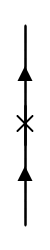
\includegraphics[height=3cm]{figures/diagramA.png}
		\caption{Diagram A}
	\end{subfigure}
	\begin{subfigure}{0.2\textwidth}
		\centering
		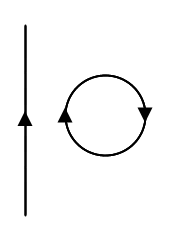
\includegraphics[height=3cm]{figures/diagramB.png}
		\caption{Diagram B}
	\end{subfigure}
	\begin{subfigure}{0.2\textwidth}
		\centering
		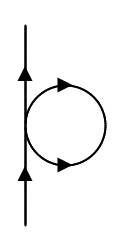
\includegraphics[height=3cm]{figures/diagramC.png}
		\caption{Diagram C}
	\end{subfigure}
	\begin{subfigure}{0.2\textwidth}
		\centering
		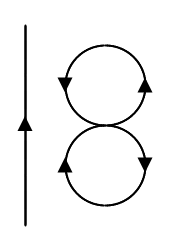
\includegraphics[height=3cm]{figures/diagramD.png}
		\caption{Diagram D}
	\end{subfigure}
\end{figure}

Additionally, we find that in the $w_{rs}$ case (A and B), there is always one incoming line and one outcoming line for each intermediate vertex, which is because of one creation operator and one annihilation operator in the expression $W=w_{rs} c_r^{\dagger} c_s$.
In the $V_{uvrs}$ case (C and D), there are always two incoming lines and two outcoming lines for each intermediate vertex, which is because of two creation operators and two annihilation operators in the expression $V=\frac{1}{2}V_{uvrs} c_u^{\dagger} c_v^{\dagger} c_s c_r$.

Compared with the expressions, the diagrams are very simple, which is one of its advantages.
In fact, Feynman diagram can not only show the structure of expression, but can also restore all the algebraic details.
This means that, instead of doing any algebraic calculation, we can just draw all the possible diagrams and then use some rules to translate to algebraic results.
Then we will derive the rules:

For each vertex, we assign $w_{rs}$ or $V_{uv[rs]}$ depending on whether it's a $w$ vertex or a $V$ vertex:

\hspace{0.2\textwidth}
\begin{minipage}{0.08\textwidth}
	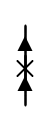
\includegraphics[height=3cm]{figures/vertexW.png}
\end{minipage}
\begin{minipage}{0.2\textwidth}
	$=w_{rs}$
\end{minipage}
\begin{minipage}{0.18\textwidth}
	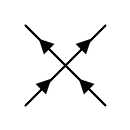
\includegraphics[height=3cm]{figures/vertexV.png}
\end{minipage}
\begin{minipage}{0.1\textwidth}
	$=V_{uv[rs]}$
\end{minipage}

It is easy to understand the result of $w$ vertex, since $W=w_{rs} c_r^{\dagger} c_s$.
For the $V$ case, $V=\frac{1}{2}V_{uvrs} c_u^{\dagger} c_v^{\dagger} c_s c_r$.
Wick's theorem states all possible of contraction should be included, thus any algebraic expression will have "partners" that the only difference is the exchange of index $u$ and $v$, or $s$ and $r$, or both.
Thus, instead of $\frac{1}{2}V_{uvrs}$, the proper magnitude should be $\frac{1}{2}V_{[uv][rs]}=V_{uv[rs]}$.

However, it is not always the case, since sometimes we will meet double counting.
For example in the double loop in Diagram D, which corresponds to algebraic expression
\begin{equation}
	\langle\Phi_{0}|
	\hat{\mathcal{T}}\left[
		c_{u}^{\dagger}\left(t_{1}\right) 
		c_{v}^{\dagger}\left(t_{1}\right)
		c_{s}\left(t_{1}\right) 
		c_{r}\left(t_{1}\right)
	\right]
	| \Phi_{0}\rangle
\end{equation}

Obviously, there is only two contraction schemes, i.e. $u$ with $s$, $v$ with $r$, or $u$ with $r$, $v$ with $s$. 
Thus, we meet double counting here.
Generally, when two lines are equal, double counting happens.
Thus, the final result should be divided by two for each pair of equal lines.


Each line or curve is assigned by its corresponding Green function, which is also easy to understand.
In the case of higher orders, the expression is 
\begin{equation} \label{greenexp}
\begin{aligned}
	i \tilde{G}^n_{p q}\left(t, t^{\prime}\right)
	=& \frac{(-i)^{n}}{n !} 
	\int_{-\infty}^{\infty} \mathrm{d} t_{1} e^{-\epsilon|t_{1}|} \ldots \int_{-\infty}^{\infty} \mathrm{d} t_{n} e^{-\epsilon|t_{n}|}
	\\
	& \langle\Phi_{0}|
	\hat{\boldsymbol{T}}\left[\hat{H}_{I}\left(t_{1}\right) \ldots \hat{H}_{I}\left(t_{n}\right) c_{p}(t) c_{q}^{\dagger}\left(t^{\prime}\right)\right]|
	\Phi_{0}\rangle
\end{aligned}
\end{equation}
which has a factor of $\frac{(-i)^n}{n!}$.

However, $t_1 \dots t_n$ are treated on each footing and can also be exchanged when calculating the time-ordered product, thus it will contribute a factor $n!$.
Thus the overall factor is $(-i)^n$.

Last but not least, we need to determine the overall sign of the expression.
Unfortunately, it is impossible to determine the sign just from diagram, thus one must go back to any one of the algebraic expressions and then count how many times one need to commute creation and annihilation operator in the expression of time-ordered product.

Feynman diagram drawn by above rules is refered as Abrikosov diagram.

Then we go back to the calculation of first order Green function.
Let's first focus on expression B and D.
Both parts contain $G^0_{pq}(t,t^{\prime})$, which corresponds to a separate line in Diagram B and D.
Now we introduce the famous linked-cluster theorem, which states that all diagrams contain a separate $G^0_{pq}(t,t^{\prime}$ line will be canceled by the denominator of Eq \ref{greenexp}.
The proof is given in the reference \cite{main}.
Here we take first order Green function as an example.

Up to the first order, Green function can be written as
\begin{equation}
	\begin{aligned}
		i\tilde{G}_{pq}(t,t^{\prime})=&i \delta_{pq} G^0_{p}(t,t^{\prime})
		\\
		+&w_{pq} G^0_p(t,t_1) G^0_q(t_1,t^{\prime}) - w_{rr} G^0_r(t_1,t_1) \delta_{pq} G^0_{p}(t,t^{\prime})
		\\
		-&V_{pr[qr]} G^0_{p}(t,t_1) G^0_{r}(t_1,t_1) G^0_{q}(t_1,t^{\prime})
		- V_{rs[rs]} G^0_r(t_1,t_1) G^0_s(t_1,t_1) \delta_{pq} G^0_p(t,t^{\prime})
		\\
		+&O(2)
	\end{aligned}
\end{equation}
while the denominator is 
\begin{equation}
	\langle\Phi_{0}|\hat{U}_{\epsilon}(0,-\infty)| \Phi_{0}\rangle=1
		- w_{rr} G^0_r(t_1,t_1)
		- V_{rs[rs]} G^0_r(t_1,t_1) G^0_s(t_1,t_1)
		+ O(2)
\end{equation}

Thus up to the first order,  the overall Green function reads
\begin{equation}
	i G_{pq}(t,t^{\prime})=i \delta_{pq} G^0_{p}(t,t^{\prime})
	+w_{pq} G^0_p(t,t_1) G^0_q(t_1,t^{\prime})
	-V_{pr[qr]} G^0_{p}(t,t_1) G^0_{r}(t_1,t_1) G^0_{q}(t_1,t^{\prime}) +O(2)
\end{equation}
where all unlinked diagrams are canceled.

As we mentioned before, both the numerator and denominator contains divergent terms, which will be canceled after division.
In fact, the divergent parts are exactly the unlinked diagrams.
Thus, linked-cluster theorem decreases the number of diagrams we need to calculate, and also guarantees the result is finite and thus physical.

Then we analyze the rest terms of first order Green function:
\begin{equation}
	\begin{aligned}
		i G^1_{pq}(t,t^{\prime}) &= w_{pq} G^0_p(t,t_1) G^0_q(t_1,t^{\prime})
		-V_{pr[qr]} G^0_{p}(t,t_1) G^0_{r}(t_1,t_1) G^0_{q}(t_1,t^{\prime})
		\\
		&= G^0_p(t,t_1) G^0_q(t_1,t^{\prime}) (w_{pq}-V_{pr[qr]}G^0_r(t_1,t_1)
		\\
		&= G^0_p(t,t_1) G^0_q(t_1,t^{\prime}) (w_{pq}+V_{pr[qr]}n_r)
		\\
		&=0
	\end{aligned}
\end{equation}
where 
\begin{equation}
	\begin{aligned}
		G^0_r(t_1,t_1)&=G^0_r(t_1,t_1^{+})
		\\
		&=- \langle\Phi_{0}|
		c_r^{\dagger} c_r
		| \Phi_{0}\rangle
		\\
		&=-n_r
	\end{aligned}
\end{equation}
is used.

In fact, the diagrams that contain $w$ vertex will always cancel with the diagrams that contain free Green function line starting and ending with the same $V$ vertex.
According to Eq \ref{greenexp}, $H_I$, which is $W$ and $V$ always appear together.
Thus, any diagram contain $V_{pr[qr]}n_r$ will automatically contain $r_{pq}$.
This result means that we can skip all diagrams with $W$ vertex and that contain free Green function line starting and ending with the same $V$ vertex at the same time.
Thus, we will not consider $W$ vertex in the following.

Then we summarize the Feynman rules for Abrikosov diagram:
\begin{itemize}
	\item Draw all topologically distinct connected diagrams with $n$ interaction dots and $2n + 1$ directed (solid) free Green’s function starting at the outer vertex $(p, t)$ and ending at the outer vertex $(q, t^{\prime})$.
		At each interaction dot, two Green function start and two end; assign a time argument to each interaction dot.
	\item Attach one-particle indices and time arguments to the free Green function lines; the arrows define the order of the time arguments. Replace the graphical symbols (free Green function lines and interaction dots) by the respective analytical expressions.
	\item Sum over indices and integrate over time arguments of the inner vertices.
	\item The overall phase of an Abrikosov diagram can only be fixed by inspecting one of the Feynman diagrams comprised in the Abrikosov diagram.
		The phase is to be adapted in such a way that this Feynman diagram is reproduced correctly by the Abrikosov expression.
	\item Apply a factor of $\frac{1}{2}$ for each pair of (topologically) equivalent free Green function lines to compensate for double counting of Feynman diagrams. Double counting may arise for other reasons at fourth and higher order, and this possibility must be checked at the level of Feynman diagrams.
\end{itemize}

We calculate the second order Green function as the end of this section:
According to the Feynman diagram, we first draw all possible topologically inequivalent diagrams.
In the case of second order Green function, there is only one diagram:
\begin{figure}[h]
	\centering
	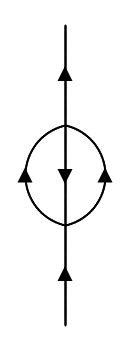
\includegraphics[height=4cm]{figures/order2.png}
	\caption{Diagram of second order Green function}
\end{figure}

Note that the two curves are identical ( start and end with the same vertices).
Thus, according the Feynman rules, we can easily determine the second order Green function up to a overall sign:
\begin{equation} \label{order2}
	\begin{aligned} 
	G_{p q}^{(2)}\left(t, t^{\prime}\right)=\pm \frac{1}{2} \sum_{r, u, v_{-\infty}} & \int_{-\infty}^{\infty} \mathrm{d} t_{1} \int_{-\infty}^{\infty} \mathrm{d} t_{2} V_{p r[u v]} V_{u v[q r]} 
	\\ 
	& G_{p}^{0}\left(t, t_{1}\right) G_{u}^{0}\left(t_{1}, t_{2}\right) G_{v}^{0}\left(t_{1}, t_{2}\right) G_{r}^{0}\left(t_{2}, t_{1}\right) G_{q}^{0}\left(t_{2}, t^{\prime}\right) 
	\end{aligned}
\end{equation}

To determine the overall sign, we only need to consider the case
\begin{equation}
	\langle\Phi_{0}|
	\hat{\mathcal{T}}\left[
		\wick{\c4 c_{u}^{\dagger}\left(t_{1}\right) \c3 c_{v}^{\dagger}\left(t_{1}\right) \c2 c_{s}\left(t_{1}\right) \c1 c_{r}\left(t_{1}\right) \c1 c_{i}^{\dagger}\left(t_{2}\right) \c2 c_{j}^{\dagger}\left(t_{2}\right) \c3 c_{l}\left(t_{2}\right) \c1 c_{k}\left(t_{2}\right) \c4 c_{p}(t) \c1 c_{q}^{\dagger}\left(t^{\prime}\right)}
		\right]
		| \Phi_{0}\rangle
\end{equation}
which gives an overall sign of $-1$, which is canceled with the factor $(-i)^2$.

Thus the overall sign of expression Eq \ref{order2} should be positive.

